% 进行了精简, 只保留一些结论

本文所有游戏若无特殊说明，均为\textbf{正常规则}的公平组合游戏（无法移动者负）。

状态分为（先手）必胜状态 $\Nw$ 与（先手）必败状态 $\Pw$（$\Nw/\Pw$ 取 Next/Previous player wins 之意）。

\subsection{Nim 游戏与博弈图}

\begin{game}[Nim]
	$n$ 堆石子，第 $i$ 堆 $a_i$ 枚。两人轮流从任意一堆取走任意多枚石子，不能不取。取走最后一枚者胜。
\end{game}

\begin{lemma}[状态分类引理]
	正常规则的公平组合游戏中：
	\begin{enumerate}
		\item 无后继状态的状态是必败状态 $\Pw$；
		\item 状态为 $\Nw$ 当且仅当它存在至少一个后继为 $\Pw$；
		\item 状态为 $\Pw$ 当且仅当它的所有后继均为 $\Nw$。
	\end{enumerate}
	公平组合游戏的博弈图是有向无环图（每次操作总量严格减少），逆拓扑递推可在 $O(|V|+|E|)$ 内完成全部状态的 $\Nw/\Pw$ 分类。直接对 Nim 画博弈图则需 $\Omega\!\left(\prod_{i=1}^n(a_i+1)\right)$，不可行。
\end{lemma}

\begin{figure}[htbp]
	\centering
	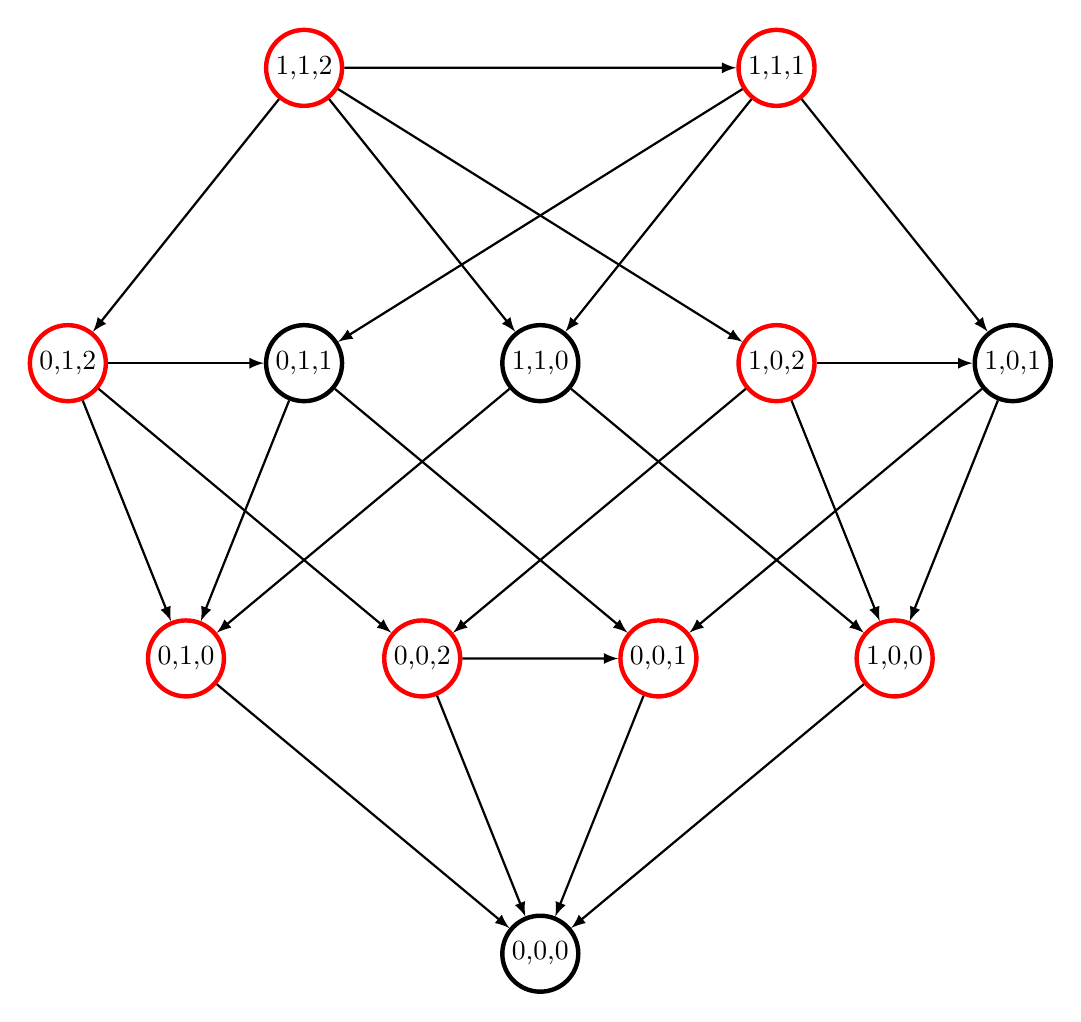
\begin{tikzpicture}[
		xscale=1.5, yscale=1.25,
		every node/.style={circle, ultra thick, draw, inner sep=2pt},
		every path/.style={thick, ->, >=latex},
		]
		\node[draw=red] (112) at (-2, 3) {1,1,2};
		\node[draw=red] (111) at ( 2, 3) {1,1,1};
		\node[draw=red] (012) at (-4, 0) {0,1,2};
		\node[draw=black] (011) at (-2, 0) {0,1,1};
		\node[draw=black] (110) at ( 0, 0) {1,1,0};
		\node[draw=red] (102) at ( 2, 0) {1,0,2};
		\node[draw=black] (101) at ( 4, 0) {1,0,1};
		\node[draw=red] (010) at (-3,-3) {0,1,0};
		\node[draw=red] (002) at (-1,-3) {0,0,2};
		\node[draw=red] (001) at ( 1,-3) {0,0,1};
		\node[draw=red] (100) at ( 3,-3) {1,0,0};
		\node[draw=black] (000) at ( 0,-6) {0,0,0};
		\path (112) edge (012);
		\path (012) edge (002);
		\path (002) edge (001);
		\path (001) edge (000);
		\path (002) edge (000);
		\path (012) edge (011);
		\path (011) edge (001);
		\path (011) edge (010);
		\path (010) edge (000);
		\path (012) edge (010);
		\path (112) edge (102);
		\path (102) edge (002);
		\path (102) edge (101);
		\path (101) edge (001);
		\path (101) edge (100);
		\path (100) edge (000);
		\path (102) edge (100);
		\path (112) edge (111);
		\path (111) edge (011);
		\path (111) edge (101);
		\path (111) edge (110);
		\path (110) edge (010);
		\path (110) edge (100);
		\path (112) edge (110);
	\end{tikzpicture}
	\caption{初始局面 $(1,1,2)$ 的 Nim 博弈图。红圈为必胜状态 $\Nw$，黑圈为必败状态 $\Pw$。}
\end{figure}

\newpage

\begin{definition}[Nim 和]
	$a_1\oplus a_2\oplus\cdots\oplus a_n$（按位异或）。
\end{definition}

\begin{theorem}[Nim 游戏判定]
	$ (a_1,a_2,\cdots,a_n)\in\Pw \iff a_1\oplus a_2\oplus\cdots\oplus a_n=0. $
\end{theorem}

\begin{proof}[证明（同时给出必胜策略）]

	对所有可能的状态应用归纳法：
	
	\begin{enumerate}
		\item 如果 $a_i=0$ 对所有 $i=1,\cdots,n$ 都成立，该状态没有后继状态，且 Nim 和等于 $0$，命题成立．
		
		\item 如果 $k = a_1\oplus a_2\oplus\cdots\oplus a_n\neq 0$，那么，需要证明该状态是必胜状态．也就是说，需要构造一个合法移动，使得后继状态为必败状态；由归纳假设，只需要证明后继状态满足 $a'_1\oplus a'_2\oplus\cdots\oplus a'_n=0$．利用 Nim 和（即异或）的性质，这等价于说，存在第 $i$ 堆石子，从中拿走若干枚石子后，数量可以变为 $a_i\oplus k$，亦即 $a_i>a_i\oplus k$．
		
		实际上，设 $k$ 的二进制表示中，最高位的 $1$ 是第 $d$ 位．那么，一定存在某个 $a_i$，使得它的二进制第 $d$ 位是 $1$．对于相应的石子堆，就一定有 $a_i>a_i\oplus k$，因为 $a_i\oplus k$ 中第 $d$ 位为 $0$，更高位和 $a_i$ 一样．
		
		\item 如果 $a_1\oplus a_2\oplus\cdots\oplus a_n= 0$，那么，需要证明该状态是必败状态．由归纳假设可知，只要证明它的所有后继状态的 Nim 和都不是 $0$．这是必然的，任何合法移动将 $a_i$ 变为 $a'_i\neq a_i$，就必然会使得 Nim 和变为 $a'_i\oplus a_i\neq 0$．
	\end{enumerate}
\end{proof}

\subsection{常见公平游戏结论速查}

本节结论的证明均为验证式：只需验证「从 $\Pw$ 出发只能到 $\Nw$；从 $\Nw$ 出发总能到某个 $\Pw$」，再对博弈图归纳即严格。

\subsubsection{Bachet 游戏}
\begin{game}[Bachet]
	一堆 $n$ 枚石子，每次取 $1\sim k$ 枚，取走最后一枚者胜。
\end{game}
\begin{theorem}
	$\Pw \iff n\equiv0\pmod{k+1}$；且 $\SG(n)=n\bmod(k+1)$。
\end{theorem}
必胜策略：取走 $n\bmod(k+1)$ 枚使余数归零；对手取 $k'$ 枚后自己取 $k+1-k'$ 枚。

\subsubsection{Moore's Nim-$k$ 游戏}
\begin{game}[Moore's Nim-$k$]
	$n$ 堆石子，每次可从至少 $1$ 堆、至多 $k$ 堆中各取任意多枚（不能不取），取走最后一枚者胜。
\end{game}
\begin{theorem}
	把每堆石子数写成二进制，对每个数位 $d$ 统计「第 $d$ 位为 $1$ 的堆数」模 $(k+1)$ 的余数。所有数位的余数全为 $0$ $\iff$ $\Pw$，否则 $\Nw$。$k=1$ 时即普通 Nim。
\end{theorem}

\newpage

\subsubsection{阶梯 Nim 游戏}
\begin{game}[阶梯 Nim]
	$n$ 堆石子排成一列。每次要么取走第 $1$ 堆中任意多枚，要么把第 $i>1$ 堆中任意多枚移到第 $i-1$ 堆，不能不动。取走最后一枚者胜。
\end{game}
\begin{theorem}
	$$\Pw \iff a_1\oplus a_3\oplus\cdots\oplus a_{n-1+(n\bmod 2)}=0\quad(\text{只看奇数号堆}).$$
\end{theorem}
直觉：偶数堆移向奇数堆的操作会被对手原样继续下移/取走而抵消，故等价于奇数号堆上的普通 Nim。

\subsubsection{Fibonacci Nim 游戏}
\begin{game}[Fibonacci Nim]
	一堆 $n$ 枚石子。先手第一步可取任意多枚但不能取完；之后每步所取不得超过对手上一步所取的两倍，且不得为 $0$。取走最后一枚者胜。
\end{game}
\begin{theorem}[Zeckendorf]
	记 $q$ 为当前回合限额（首回合 $q=n-1$，之后为对手上步所取的二倍）。当前状态 $\Nw \iff q\ge n$ 的 Fibonacci 分解（Zeckendorf 表示：分解为互不相邻的正 Fibonacci 数之和）中的最小项。特别地，开局 $\Pw \iff n$ 本身是 Fibonacci 数。
\end{theorem}

\subsubsection{Wythoff 游戏}
\begin{game}[Wythoff]
	两堆石子 $a_1,a_2$。每次从一堆取任意多枚，或从两堆取相同数目，不能不取。取走最后一枚者胜。
\end{game}
\begin{theorem}
	设 $a_1\le a_2$，$\phi=\dfrac{\sqrt5+1}{2}$，则
	$$\Pw \iff a_1=\big\lfloor(a_2-a_1)\,\phi\big\rfloor.$$
	即必败态恰为 $(\lfloor k\phi\rfloor,\ \lfloor k\phi^2\rfloor)=(\lfloor k\phi\rfloor,\ \lfloor k\phi\rfloor+k)$，$k\in\N$。
\end{theorem}
\begin{lemma}[Beatty--Rayleigh]
	无理数 $r,s>1$ 满足 $\frac1r+\frac1s=1$，则 Beatty 序列 $\mathcal B_r=\{\lfloor kr\rfloor:k\in\N_+\}$ 与 $\mathcal B_s$ 构成 $\N_+$ 的分划。Wythoff 中取 $r=\phi,\ s=\phi+1=\phi^2$。
\end{lemma}

\subsubsection{翻硬币游戏}
\begin{game}[翻硬币]
	$(S,\preceq)$ 为良基偏序集，$f:S\to\mathcal{P}\mathcal{P}S$ 满足：对所有 $s$，$f(s)$ 非空；$T\in f(s)\Rightarrow s\in T$；$t\in T\Rightarrow t\preceq s$。$S$ 每处放一枚硬币（正面或背面朝上）。每步选一枚正面硬币 $s$ 与集合 $T\in f(s)$，翻转 $T$ 中所有硬币。把硬币全部翻成背面者胜。
\end{game}
\begin{theorem}
	设 $G_s$ 为仅 $s$ 处硬币正面的基础局面，$H(G)\subseteq S$ 为局面 $G$ 中正面位置的集合，则
	$$\SG(G)=\bigoplus_{s\in H(G)}\SG(G_s),\qquad
	\SG(G_s)=\mex_{T\in f(s)}\ \bigoplus_{t\in T\setminus\{s\}}\SG(G_t).$$
\end{theorem}
要点：每枚正面硬币是一个独立子游戏，整体是它们的和；同一位置翻回正面相当于「复制」已有子游戏，异或下两两抵消，故 SG 值只取决于正面位置的集合。

\subsubsection{二分图博弈（无向图删点游戏）}
\begin{game}[二分图博弈]
	局面为 $(G,v)$，$G=(V,E)$ 无向图，$v\in V$。当前玩家选一个与 $v$ 相邻的顶点 $u$，从图中删去 $v$ 及其所有关联边，新局面 $(G',u)$ 交给对手。轮到时 $v$ 无相邻顶点者负。
\end{game}
\begin{theorem}
	先手必胜 $\iff$ $v$ 是 $G$ 的最大匹配关键点（出现在 $G$ 的所有最大匹配中）。结论对一般无向图成立，与二分结构无关。
\end{theorem}
\begin{corollary}[变体：相邻取石子]
	每个顶点放一枚石子，先手任取一枚起步，之后每步所取顶点须与对手上一步所取相邻。先手必败 $\iff$ 每个顶点都是最大匹配关键点 $\iff$ $G$ 存在完美匹配。
\end{corollary}

\subsection{反常（Mis\`ere）Nim 游戏}

规则同 Nim，但取走最后一枚石子者\textbf{负}。
\begin{theorem}
	$(a_1,a_2,\cdots,a_n)\in\Pw$ 当且仅当：
	\begin{enumerate}
		\item 存在 $a_i>1$，且 $a_1\oplus a_2\oplus\cdots\oplus a_n=0$；或
		\item 所有 $a_i\le1$，且非空堆数为奇数。
	\end{enumerate}
\end{theorem}
即：存在多于一枚的堆时结论与正常 Nim 一致；全为单枚堆时奇偶反转。

\subsection{有向图游戏（允许有环，含平局）}

沿有向边轮流移动，无法移动者按正常/反常规则判负/判胜；游戏可能永不终止（平局）。分类规则：
\begin{itemize}
	\item 有后继的状态：$\Nw \iff$ 存在后继为 $\Pw$；$\Pw \iff$ 所有后继为 $\Nw$；
	\item 无法归入上两类的状态为平局。
\end{itemize}
逆拓扑（retrograde）算法，$O(|V|+|E|)$：
\begin{enumerate}
	\item 记录所有状态出度；出度为 $0$ 的状态入队，按正常/反常规则分别设为 $\Pw$/$\Nw$；
	\item 弹出队首：若为 $\Pw$，把所有未判定前驱设为 $\Nw$ 并入队；若为 $\Nw$，把其前驱出度各减一，出度归零的前驱设为 $\Pw$ 并入队；
	\item 队列空即终止；仍未判定的状态全是平局。
\end{enumerate}